\documentclass[10pt,twocolumn,letterpaper]{article}

% ---------------------------------------------------------------- packages
\usepackage[T1]{fontenc}
\usepackage[utf8]{inputenc}
\usepackage{newtxtext,newtxmath}
\usepackage[margin=0.75in,columnsep=0.25in]{geometry}
\usepackage{graphicx}
\usepackage{booktabs}
\usepackage{multirow}
\usepackage{array}
\usepackage{xcolor}
\usepackage{enumitem}
\usepackage[font=small,labelfont=bf,skip=4pt]{caption}
\usepackage{subcaption}
\usepackage[numbers,sort&compress]{natbib}
\usepackage{microtype}
\usepackage[colorlinks=true,linkcolor=blue!50!black,citecolor=blue!50!black,urlcolor=blue!50!black]{hyperref}

\graphicspath{{figures/}}
\setlist{nosep,leftmargin=*}
\newcommand{\repo}{\url{https://github.com/KirkEHaskell/delta-robot-act-vs-diffusion}}
\newcommand{\hf}{\url{https://huggingface.co/KirkHaskell}}
\newcommand{\best}[1]{\textbf{#1}}

\title{\Large\bfseries ACT vs.\ Diffusion Policy on a Home-Built Delta Robot:\\
Data and Training-Length Scaling for Real-World Pick-and-Place}
\author{Kirk Haskell\thanks{Independent project, carried out outside of coursework and not
supported or endorsed by Tufts University.}\\[1pt]
\small Tufts University\\[2pt]
\small Code, CAD, firmware, data and models: \repo}
\date{October 2026}

\begin{document}
\maketitle

% ================================================================ abstract
\begin{abstract}
We compare the two most widely used open-source imitation-learning policies, ACT and Diffusion
Policy, on a home-built 3-DOF delta robot with an electromagnet gripper performing a bolt
pick-and-place task. Both policies are trained on nested subsets of 10, 25, 50 and 100
teleoperated demonstrations for 5k, 20k and 50k optimizer steps, giving 24 models. Each model is
scored on 10 real-robot trials, for 240 trials in total. Out of the box, LeRobot's Diffusion
Policy never left its start pose. Input-ablation tests showed that it had learned to copy the
robot's own joint state, a shortcut that leader--follower teleoperation data makes nearly
optimal. An ImageNet-pretrained encoder, crop augmentation, a blinded joint-state input and a
1.6\,s action horizon fixed it. With these changes the best model, Diffusion Policy with 100
demonstrations and 50k steps, succeeded on \best{10/10} trials; the best ACT models reached 6/10.
Neither policy is usable with 10 demonstrations or 5k steps. ACT shows a clean data-scaling
trend at 50k steps ($0\rightarrow 20\rightarrow 50\rightarrow 60\%$, $p=0.0015$). Pooled over the
grid, the two policies are not significantly different (39/120 vs.\ 29/120, $p=0.20$). They fail
differently: ACT knocks the bolt over, Diffusion Policy stalls. We release the dataset, the trial
log, all code, CAD and firmware, and the two best checkpoints.
\end{abstract}

% ================================================================ 1
\section{Introduction}

Imitation learning from teleoperated demonstrations has become the default way to teach low-cost
robot arms manipulation skills. In open-source practice two policy classes dominate:
ACT~\cite{zhao2023act} and Diffusion Policy~\cite{chi2023diffusion}, both available in Hugging
Face's LeRobot library~\cite{cadene2024lerobot}. A practitioner adopting either one faces two
immediate questions: \emph{how many demonstrations are needed}, and \emph{how long to train}.

Published comparisons mostly report one data and compute setting on standard serial arms. This
study measures a full $4\times3$ grid of data and training length for both policies, on a
mechanically different robot, a parallel (delta) robot with a binary magnetic gripper, and scores
every model on the real robot under a fixed protocol.

\paragraph{Contributions.}
\begin{itemize}
  \item A controlled real-robot grid: 2 policies $\times$ 4 data sizes $\times$ 3 training lengths,
        240 scored trials, released with the raw trial log and the code that regenerates every
        number and figure.
  \item A documented failure of default Diffusion Policy on leader--follower data, an instance of
        the ``copycat'' problem~\cite{wen2020copycat}; an offline diagnostic that detects it in
        minutes, and a fix.
  \item An open 100-episode, 3-camera dataset in LeRobot v3.0 format for a delta-robot embodiment,
        which is rare in public robot-learning data.
  \item Open hardware (STL and URDF), firmware, and recording and evaluation software.
\end{itemize}

\begin{figure}[t]
  \centering
  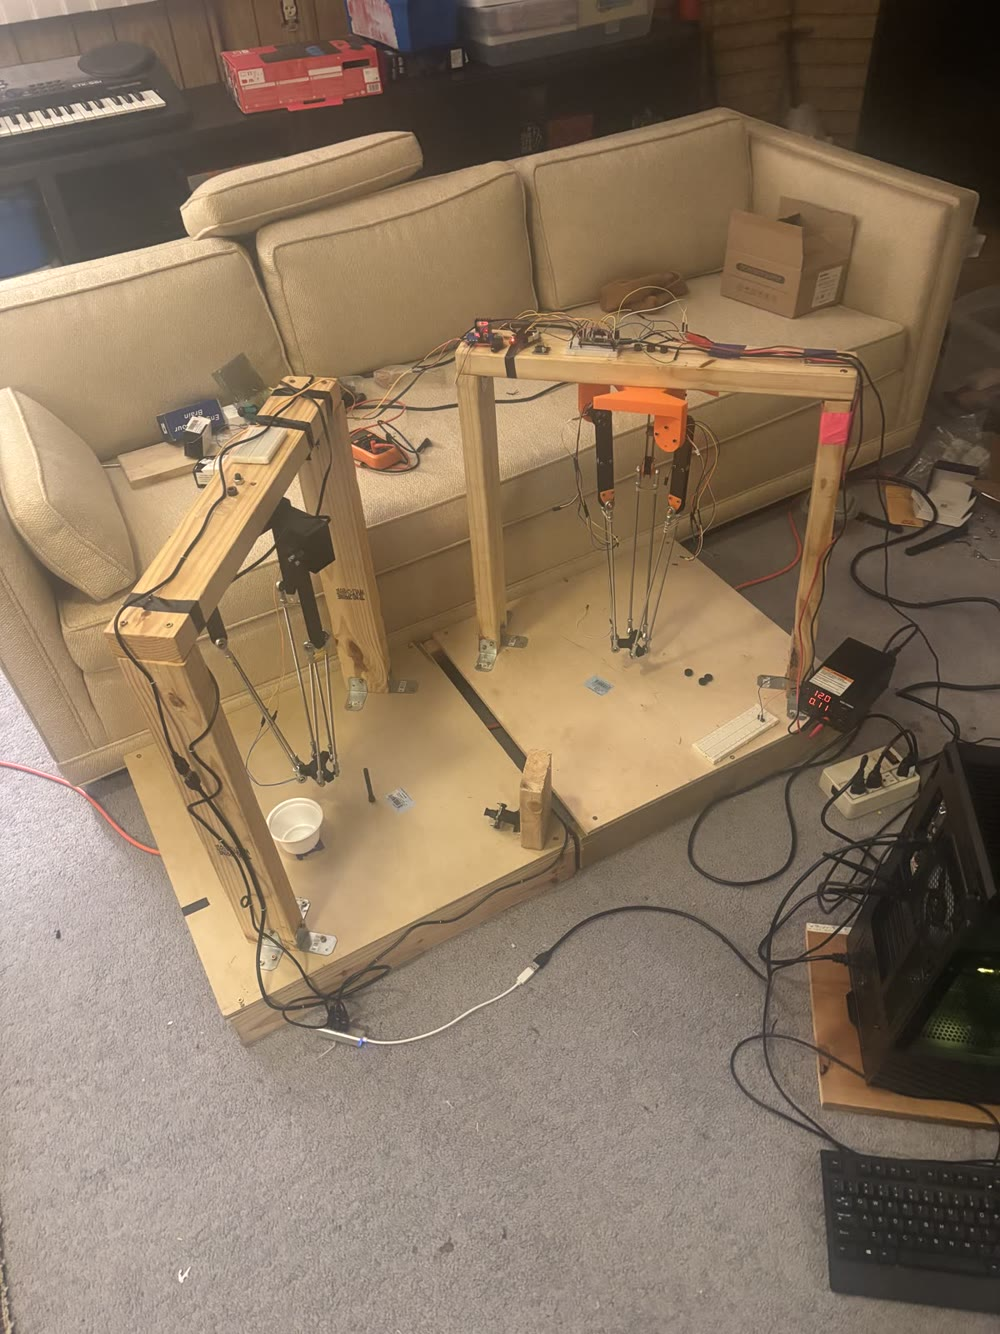
\includegraphics[width=\columnwidth]{robots.jpg}
  \caption{The two robots. \textbf{Left:} the servo-driven follower that the policies control,
  with the cup and a standing bolt. \textbf{Right:} the hand-moved leader arm used for
  teleoperation, with a magnetic encoder at each shoulder joint.}
  \label{fig:robots}
\end{figure}

% ================================================================ 2
\section{Related Work}

\textbf{ACT}~\cite{zhao2023act} encodes camera images with a ResNet-18~\cite{he2016resnet} and
predicts chunks of future actions with a conditional-VAE transformer. \textbf{Diffusion
Policy}~\cite{chi2023diffusion} predicts an action sequence by iterative denoising
(DDPM~\cite{ho2020ddpm}; DDIM~\cite{song2021ddim} for faster sampling) conditioned on a short
observation history. Both are implemented in LeRobot~\cite{cadene2024lerobot}, which we use
throughout.

Behaviour cloning is known to latch onto spurious, easily predicted signals. Causal
confusion~\cite{dehaan2019causal} and the copycat problem~\cite{wen2020copycat} describe policies
that infer the next action from their own previous actions or state history instead of from the
task-relevant observation, a form of shortcut learning~\cite{geirhos2020shortcut}. We observe
this effect concretely on real hardware with an off-the-shelf implementation, and show how a
specific property of leader--follower data triggers it.

% ================================================================ 3
\section{System}

\paragraph{Robot.} A 3-DOF delta robot. Three printed upper arms are driven by Feetech STS3215
serial-bus servos; steel parallelogram rods with ball joints carry the end effector. The gripper
is an electromagnet ($\sim$12\,V) switched through an H-bridge, which lifts a standing steel bolt.
A Teensy~4.1 drives the servo bus at 1\,Mbit/s. Joint commands are absolute angles in degrees,
clamped to $[30^\circ, 110^\circ]$.

\paragraph{Teleoperation.} Demonstrations are collected leader--follower
(Fig.~\ref{fig:robots}): a second, passive delta arm carries an AS5600 magnetic encoder on each
shoulder, and the Teensy drives the follower servos to the leader's angles in real time. A push
button switches the magnet. The Teensy streams leader angles, follower angles and magnet state at
60\,Hz; the recorder samples at 30\,Hz.

\paragraph{Cameras.} Three Innomaker U20CAM-720P USB cameras (\texttt{side}, \texttt{top\_right},
\texttt{top\_left}, Fig.~\ref{fig:cams}) are captured at $320\times240$, 30\,fps. Three
uncompressed streams saturate a single USB hub, so capture forces MJPG through PyAV, and cameras
are addressed by physical USB port rather than OS index. In all recorded data the \texttt{side}
and \texttt{top\_right} cameras have a constant yellow-green cast. Their auto white balance was
off (4600\,K) and exposure fixed at $2^{-6}$\,s, a setting left behind by an earlier script and
persisted by the Windows driver. For evaluation on Linux the same settings were reproduced through
V4L2 controls and verified against the training video's luma and chroma statistics.

\begin{figure}[t]
  \centering
  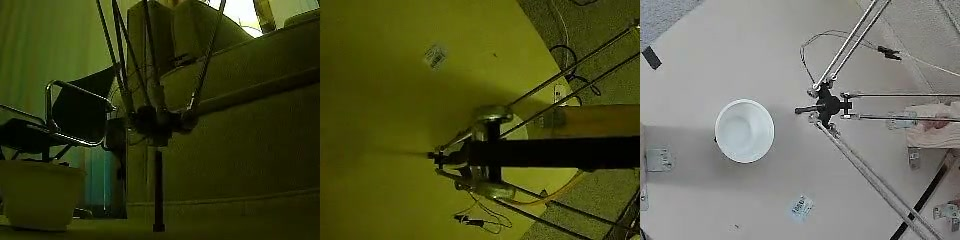
\includegraphics[width=\columnwidth]{camera_views.jpg}
  \caption{The policy's input: one frame of demonstration 42 from the \texttt{side},
  \texttt{top\_right} and \texttt{top\_left} cameras ($320\times240$ each). Note the colour cast
  on the first two, constant across the dataset.}
  \label{fig:cams}
\end{figure}

% ================================================================ 4
\section{Dataset}

The dataset contains 100 demonstrations (33{,}200 frames at 30\,Hz, 8.1--17.3\,s each, median
10.7\,s), recorded by one operator on one day in ten sessions of ten. The observation is the
follower's three joint angles plus three RGB images; the action is the leader's three joint
angles plus the magnet command (Table~\ref{tab:dataset}).

\begin{table}[t]
  \centering\small
  \caption{Dataset summary (LeRobot v3.0, AV1 video, $\sim$600\,MB).}
  \label{tab:dataset}
  \begin{tabular}{@{}l>{\raggedright\arraybackslash}p{0.66\columnwidth}@{}}
    \toprule
    Episodes / frames & 100 / 33{,}200 at 30\,Hz \\
    Observation & 3 follower joint angles (deg); 3 RGB images $240\times320$ \\
    Action & 3 leader joint angles (deg) + magnet $\{0,1\}$ \\
    Task string & ``pick up the bolt and drop it in the bucket'' \\
    Grasps & exactly one magnet press in 99/100 episodes \\
    Start pose & $(91.7, 93.2, 90.8)^\circ$, s.d.\ $\approx3.5^\circ$ per joint \\
    \bottomrule
  \end{tabular}
\end{table}

Two properties matter for learning. First, every episode opens with $\sim$1.2\,s of stillness
(median 1.23\,s) and pauses $\sim$0.33\,s after the grasp. Second, because the action is the
leader's angle and the state is the follower's, the action is always within a fraction of a
degree of the next observed state. Section~\ref{sec:copycat} shows why the second property matters.

\paragraph{Subsets.} Training subsets are nested and seeded: the episodes are shuffled with a
fixed seed and the first $N$ are taken, so $\mathcal{D}_{10}\subset\mathcal{D}_{25}\subset
\mathcal{D}_{50}\subset\mathcal{D}_{100}$ (3{,}219 / 8{,}380 / 16{,}326 / 33{,}200 frames).

% ================================================================ 5
\section{Training}

All models use LeRobot 0.5.0, PyTorch 2.6 in fp32, batch size 32, seed 1000 and a single RTX 3090.
Batch size 32 was the largest at which Diffusion Policy fits in 24\,GB. Passes over the data range
from 5 epochs (100 demos, 5k steps) to 497 (10 demos, 50k steps).

\paragraph{ACT.} LeRobot defaults: ImageNet-pretrained ResNet-18, one observation frame, chunk
size 100 with all 100 actions executed before re-planning, VAE with KL weight 10, and a constant
learning rate of $10^{-5}$. Because the learning rate is constant, one 50k-step run per data size
supplies the 5k and 20k cells as intermediate checkpoints.

\paragraph{Diffusion Policy.} The cosine learning-rate schedule depends on the total number of
steps, so each of the 12 cells is a separate run. The LeRobot defaults (``v1'') did not work on
the robot (Section~\ref{sec:copycat}). All scored Diffusion results use the ``v2'' configuration
in Table~\ref{tab:v2}; everything else (subsets, batch size, seed, schedule) matches v1.

\begin{table}[t]
  \centering\small
  \caption{Diffusion Policy: LeRobot defaults (v1) vs.\ the configuration used for all scored
  results (v2). The 48/24 horizon reproduces the original paper's 1.6\,s\,/\,0.8\,s at 30\,Hz.}
  \label{tab:v2}
  \footnotesize\setlength{\tabcolsep}{4pt}
  \begin{tabular}{@{}lll@{}}
    \toprule
    & v1 (default) & v2 \\
    \midrule
    Vision encoder & ResNet-18, scratch, GroupNorm & ImageNet, BatchNorm \\
    Augmentation & none & random crop $216\times288$ \\
    Observation frames & 2 & 1 \\
    Joint state & used & \textbf{zeroed} (train + test) \\
    Horizon / executed & 16 / 8 (0.53\,s) & 48 / 24 (1.6\,s) \\
    \bottomrule
  \end{tabular}
\end{table}

\paragraph{Training loss.} All 28 grid runs completed and their loss decreased throughout
(Fig.~\ref{fig:loss}). For both policies, \emph{fewer} demonstrations gave \emph{lower} final
loss (memorization), the opposite of the robot-success ordering. ACT's loss (L1 + KL) and
Diffusion's (noise-prediction MSE) are not comparable with each other.

\paragraph{A LeRobot 0.5.0 bug.} With episode subsets, Diffusion's episode-aware sampler yields
absolute frame indices into a dataset indexed relative to the subset. Training then crashes or
silently reads the wrong frames. A small wrapper that remaps the indices (released) was used for
every run.

\begin{figure*}[t]
  \centering
  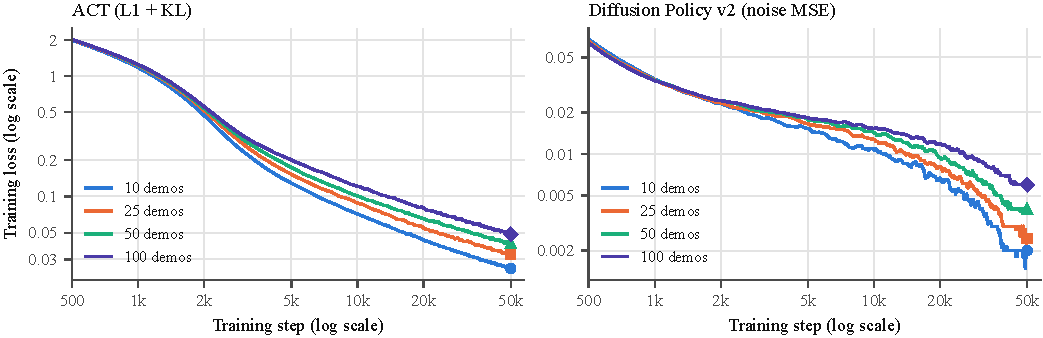
\includegraphics[width=\textwidth]{training_loss.pdf}
  \caption{Training loss of the 50k-step runs from step 500 onward (lightly smoothed, log--log axes). Fewer
  demonstrations always reach a lower loss, while robot success moves the other way
  (Fig.~\ref{fig:grid}). Losses are not comparable across the two panels.}
  \label{fig:loss}
\end{figure*}

% ================================================================ 6
\section{The Copycat Failure of Default Diffusion Policy}
\label{sec:copycat}

\paragraph{Symptom.} On the real robot every v1 Diffusion checkpoint held still at its start pose.
Changing the inference setup did not help: GPU or CPU, DDPM-100 or DDIM-10, fixed initial noise,
longer executed chunks, or a scripted ``kick-start'' lift, after which the arm stopped again. ACT
on the same rig moved normally.

\paragraph{Diagnosis.} We probed checkpoints offline on training episodes:
\begin{itemize}
  \item \emph{Teacher-forced replay} looked perfect ($\sim$0.4$^\circ$ error), so it reveals nothing.
  \item \emph{Images only} (images play the demonstration, joint state frozen at frame 0): ACT
        reproduced 92\% of the demonstrated motion range, v1 Diffusion only 37\%.
  \item \emph{State only} (images frozen, state moving): v1 Diffusion followed the state.
  \item \emph{Still start} (robot at rest, first camera frame): v1 Diffusion (50 demos, 50k steps)
        commanded $<1^\circ$ of motion, and longer training made this worse.
\end{itemize}
The policy had learned ``next action $\approx$ current joint state (+ velocity from the two
observation frames)''. With leader--follower data this is a near-perfect predictor over a short
horizon, and a still robot then predicts a still robot. The v1 defaults favour this shortcut:
a vision encoder trained from scratch, no augmentation, two state frames that expose velocity,
and a 0.53\,s horizon. ACT's pretrained encoder, single frame and 3.3\,s chunks push it towards
the images.

\paragraph{Fix.} Figure~\ref{fig:copycat} shows the pilot variants (50 demos, 5k steps).
Pretrained vision with crop augmentation barely helped (42\%). \emph{Blinding the joint state} was
decisive (96\%): the policy moved and grasped, but jittered and hesitated. Extending the horizon
to 1.6\,s removed most of the jitter, and this v2 pilot completed a pick-and-place. Fully trained
v2 models were 99--100\% image-driven by this measure.

\begin{figure}[t]
  \centering
  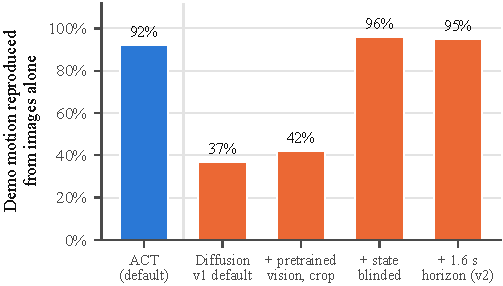
\includegraphics[width=\columnwidth]{copycat_ablation.pdf}
  \caption{Images-only ablation: the share of the demonstrated motion range a policy reproduces
  when the joint state is frozen and only the images move. Diffusion bars are cumulative changes
  to the LeRobot defaults (50 demos, 5k steps).}
  \label{fig:copycat}
\end{figure}

% ================================================================ 7
\section{Robot Evaluation}

\paragraph{Protocol.} Five bolt positions are marked on the table. P1--P3 lie inside the
demonstrated region. P4 lies inside it but is partly hidden by the cup and awkward to reach. P5
lies outside the demonstrated region but is easy to reach. Each model receives two trials per
position (10 per model). The cup position, lighting and camera setup are fixed, and models are
tested in a seeded random order. Each trial starts from the dataset's mean start pose and runs at
30\,Hz until the operator stops it or 900 actions (30\,s of motion) elapse. Success means the
bolt ends in the cup. The operator also logged whether the bolt was picked up, the number of
grasp attempts and a failure mode. Unsafe stops, where the operator halts erratic motion, count
as failures.

\paragraph{Inference.} ACT ran on a laptop CPU (Ryzen AI 9 HX 370, 0.1--0.37\,s per 100-action
chunk, 29.3--29.9\,Hz measured). Diffusion v2 ran on the RTX 3090 with DDPM-100 as trained,
taking $\sim$0.76\,s per 24-action plan; the robot pauses while it plans, which is acceptable for
this quasi-static task. On the laptop CPU, Diffusion would take $\sim$18\,s per plan.

\begin{table}[t]
  \centering\small
  \setlength{\tabcolsep}{4.5pt}
  \caption{Successes out of 10 trials per model. Superscripts: trials stopped as unsafe.}
  \label{tab:grid}
  \begin{tabular}{@{}r ccc c ccc@{}}
    \toprule
    & \multicolumn{3}{c}{ACT} && \multicolumn{3}{c}{Diffusion Policy (v2)} \\
    \cmidrule{2-4}\cmidrule{6-8}
    Demos & 5k & 20k & 50k && 5k & 20k & 50k \\
    \midrule
    10  & $0^{10}$ & $0^{2}$ & 0        && $0^{10}$ & $0^{2}$ & 2 \\
    25  & $0^{2}$  & 6       & 2        && $1^{2}$  & \best{8} & 5 \\
    50  & $1^{4}$  & $6^{1}$ & 5        && $2^{2}$  & 4       & 1 \\
    100 & $0^{10}$ & 3       & \best{6} && $0^{2}$  & 6       & \best{10} \\
    \midrule
    Total & \multicolumn{3}{c}{29/120 (24\%)} && \multicolumn{3}{c}{39/120 (33\%)} \\
    \bottomrule
  \end{tabular}
\end{table}

\begin{figure*}[t]
  \centering
  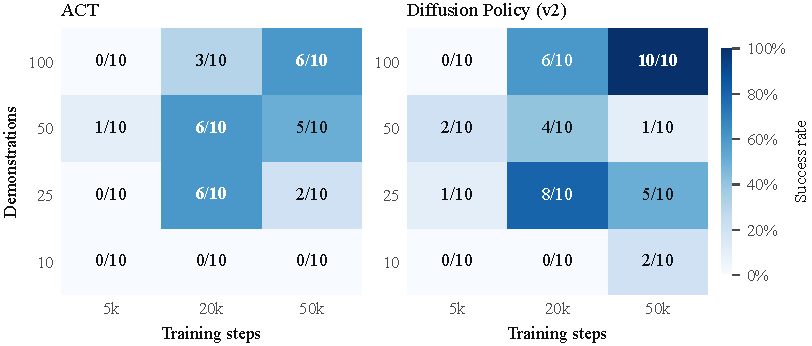
\includegraphics[width=0.8\textwidth]{success_grid.pdf}
  \caption{Real-robot success for every model (10 trials each).}
  \label{fig:grid}
\end{figure*}

\begin{figure*}[t]
  \centering
  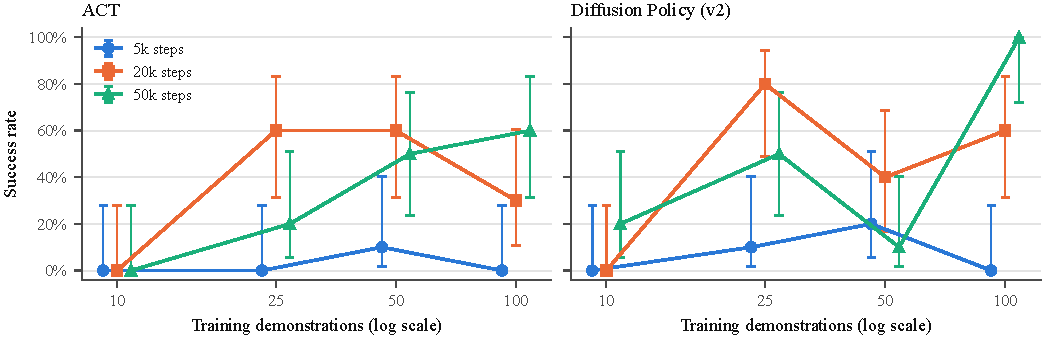
\includegraphics[width=\textwidth]{success_vs_demos.pdf}
  \caption{Success rate against the number of demonstrations, one line per training length.
  Error bars are 95\% Wilson intervals~\cite{wilson1927} ($n=10$); points are dodged
  horizontally for legibility.}
  \label{fig:demos}
\end{figure*}

\subsection{Results}

Table~\ref{tab:grid} and Fig.~\ref{fig:grid} give the full grid; Figs.~\ref{fig:demos}
and~\ref{fig:steps} show the two scaling axes. Table~\ref{tab:stats} lists the statistical
tests, with trends tested by Cochran--Armitage~\cite{armitage1955} on $\log_2$ of the varied
quantity and policy comparisons by Fisher's exact test.

\begin{table}[t]
  \centering\small
  \setlength{\tabcolsep}{3pt}
  \caption{Statistical tests (two-sided).}
  \label{tab:stats}
  \begin{tabular}{@{}lll@{}}
    \toprule
    Comparison & Successes & $p$ \\
    \midrule
    ACT, demos trend @ 50k & 0, 2, 5, 6 & 0.0015 \\
    ACT, steps trend @ 100 demos & 0, 3, 6 & 0.004 \\
    Diffusion, steps trend @ 100 demos & 0, 6, 10 & $<10^{-4}$ \\
    Diffusion, demos trend @ 50k & 2, 5, 1, 10 & 0.005$^\dagger$ \\
    ACT vs.\ Diffusion, pooled (12 cells) & 29 vs.\ 39 /120 & 0.20 \\
    ACT vs.\ Diffusion, 100 demos @ 50k & 6 vs.\ 10 /10 & 0.087 \\
    \bottomrule
    \multicolumn{3}{@{}l}{\footnotesize $^\dagger$ significant but not monotone.}
  \end{tabular}
\end{table}

\begin{figure*}[t]
  \centering
  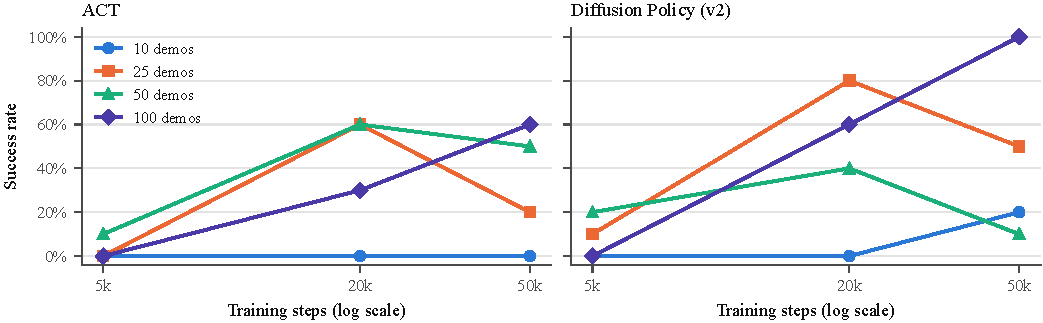
\includegraphics[width=\textwidth]{success_vs_steps.pdf}
  \caption{Success rate against training length, one line per data size.}
  \label{fig:steps}
\end{figure*}

\paragraph{Clustering caveat.} The two trials at the same position agreed in 88\% of pairs, so
each model's 10 trials carry roughly the information of 5 independent outcomes. All $p$-values
should therefore be read as optimistic, and single cells as noisy: a 6/10 cell has a 95\% interval
of 31--83\%.

\paragraph{Failure modes.} The policies fail in characteristically different ways
(Fig.~\ref{fig:outcomes}). ACT fails \emph{aggressively}: it drives to the bolt and grasps
imprecisely, knocking the standing bolt over (39 trials). Undertrained ACT at 5k steps was erratic
enough to be stopped on every trial at both 10 and 100 demonstrations. Diffusion v2 fails
\emph{hesitantly}: it hovers or freezes (52 stalls), most often before the grasp. This matches
the still segments in the demonstrations. With the state blinded, a still camera view is
ambiguous between ``about to move'' and ``waiting'', and an undertrained model can stay in the
waiting mode.

\begin{figure}[t]
  \centering
  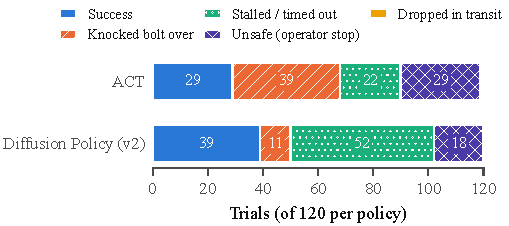
\includegraphics[width=\columnwidth]{outcomes_by_policy.pdf}
  \caption{Outcome of all 120 trials per policy.}
  \label{fig:outcomes}
\end{figure}

\paragraph{Bolt position.} P4, the occluded position, was the hardest (Fig.~\ref{fig:position}):
ACT succeeded once in 24 trials and Diffusion 7 times, and P4 accounted for 21 of the 47 unsafe
stops. The out-of-distribution position P5 was \emph{not} the hardest: both 100-demo ACT models
and the best Diffusion model went 2/2 there. Unexpectedly, both 100-demo ACT models failed at P1,
the most heavily demonstrated position, while the 50-demo ACT models succeeded there. One
untested explanation is that ACT's latent is fixed to its mean at test time, so many slightly
different P1 grasps average into one a few millimetres off, and the magnet needs near-contact.

\begin{figure}[t]
  \centering
  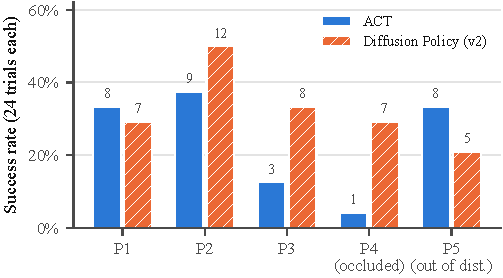
\includegraphics[width=\columnwidth]{success_by_position.pdf}
  \caption{Success by bolt position, pooled over each policy's 12 models (numbers: successes
  out of 24).}
  \label{fig:position}
\end{figure}

\paragraph{Best model.} Diffusion v2 with 100 demonstrations and 50k steps succeeded on all 10
trials, at every position including the occluded P4 and out-of-distribution P5, each with a single
grasp attempt (Fig.~\ref{fig:filmstrip}). Subjectively it was also the most convincing policy in
the study. Three ACT models reached 6/10. We release the 100-demo, 50k-step ACT as the reference
ACT model because it runs in real time on a laptop CPU and was never stopped as unsafe.

\begin{figure*}[t]
  \centering
  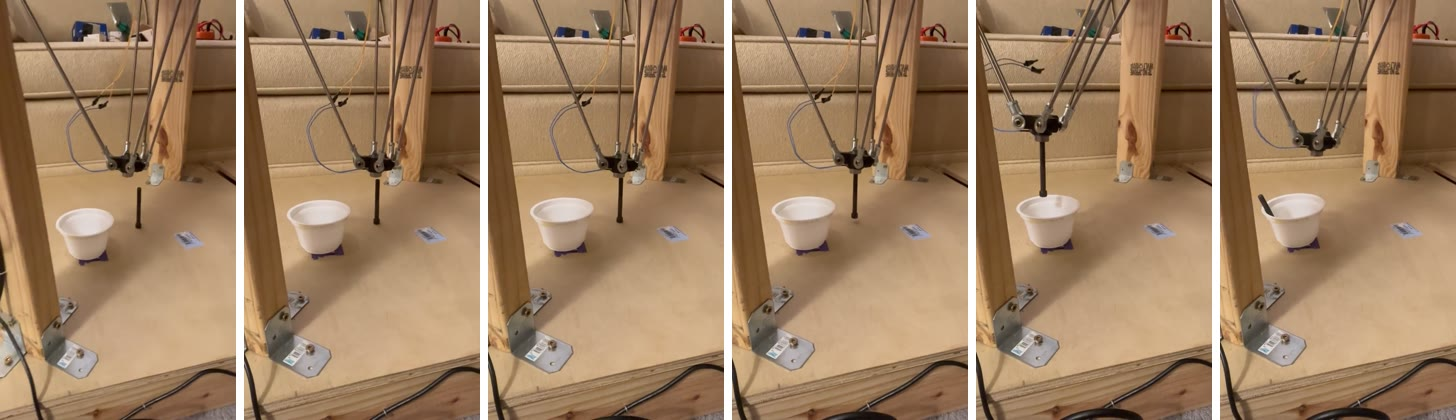
\includegraphics[width=\textwidth]{filmstrip_diffusion.jpg}
  \caption{The best model (Diffusion Policy v2, 100 demonstrations, 50k steps) completing the task
  autonomously: approach, magnetic grasp, transport, and release into the cup (frames
  $\sim$2\,s apart).}
  \label{fig:filmstrip}
\end{figure*}

% ================================================================ 8
\section{Discussion}

\paragraph{Training length is the first gate.} At 5k steps neither policy is usable (4/80 trials
combined), whatever the data size; for 100 demonstrations this is only 5 epochs. Given enough
steps, more data helps both policies, most clearly at 50k.

\paragraph{Possible overtraining at small and medium data.} At 25 demonstrations both policies did
better at 20k than at 50k steps (ACT $6\rightarrow2$, Diffusion $8\rightarrow5$), and Diffusion at
50 demonstrations fell from 4 to 1. No single drop is significant at $n=10$, but the direction
repeats three times while training loss keeps falling, and at 100 demonstrations longer training
only helped. Scaling training steps with dataset size, rather than training small datasets
longer, is a reasonable hypothesis that this data cannot confirm.

\paragraph{Policy choice is a trade-off.} Modified Diffusion Policy produced the single best model
and handled the occluded position far better. ACT was competitive in the middle of the grid,
runs in real time on a laptop CPU, and needed no changes. The pooled difference is within noise.

\paragraph{Proprioception and leader--follower data.} The same data trained ACT without trouble,
but ACT's loss of precision at P1 with 100 demonstrations hints that it may also lean on state.
A proprioception ablation for ACT is the natural next experiment. Diffusion's stalling probably
comes from the still segments in the data, so trimming them is a likely remedy. For dataset
builders the lesson is that leader--follower data invites state-copying, and that low loss or good
teacher-forced replay does not rule it out, whereas an images-only ablation does.

% ================================================================ 9
\section{Limitations}

\begin{itemize}
  \item \textbf{Unequal conditions.} ACT was evaluated on a Windows laptop CPU on 2--3 October and
        Diffusion on a Linux GPU desktop on 5 October. The random order held within each policy,
        not across them, so drift between days could align with policy.
  \item \textbf{Diffusion v2 is not stock Diffusion Policy}: it has no proprioception, pretrained
        vision, crop augmentation and a longer horizon, whereas ACT used defaults. Stock v1 was not
        formally scored; it never completed a pick in informal testing.
  \item \textbf{Small samples}: 10 trials per model, 5 positions, strong within-position clustering,
        and one training seed per cell.
  \item \textbf{Non-blind scoring}: the operator knew which model was running.
  \item \textbf{Hardware events during ACT testing}: a printed upper arm was replaced with an
        identical part; a faulty leader-encoder cable was unplugged; the firmware was patched to
        skip the missing encoders in autonomous mode; a loose magnet wire was fixed. All scored ACT
        runs logged $\sim$29.5\,Hz control.
  \item \textbf{Scene drift} between recording and testing was corrected by restoring the scene
        against the demonstration videos.
\end{itemize}

% ================================================================ 10
\section{Conclusion}

On a home-built delta robot doing pick-and-place, both ACT and Diffusion Policy need roughly
$\geq$25 demonstrations and $\geq$20k training steps before they work at all, and more data pays
off most with long training. The two policies fail in characteristically different ways. Default
Diffusion Policy can silently learn to ignore its cameras on leader--follower data; a simple
ablation exposes this and blinding proprioception fixes it, after which Diffusion Policy trained on
100 demonstrations for 50k steps solved the task in 10 of 10 trials. Future work: more trials and
seeds with blind scoring, a proprioception ablation for ACT, trimming still frames from the
demonstrations, temporal ensembling for ACT, and faster Diffusion sampling for real-time control.

\paragraph{Release.} Dataset, models: \hf. Code, CAD, firmware, trial log and figure scripts:
\repo.

\small
\bibliographystyle{unsrtnat}
\bibliography{references}

\end{document}
